\begin{frame}{Estudo de análise em regime transitório}
	\begin{itemize}
		\item \cite{Lourenco2015} discutem a abordagem de análise de estado estacionário vigente para avaliação de desempenho de sistemas computacionais
		
		\item apresenta um planejamento de experimentos de simulação destinados a análise transitória, especialmente em aplicações \textit{multi-tiers}.
	\end{itemize}
\end{frame}

\begin{frame}{Arquitetura conceitual MEDC}
	\begin{figure}
		\centering
		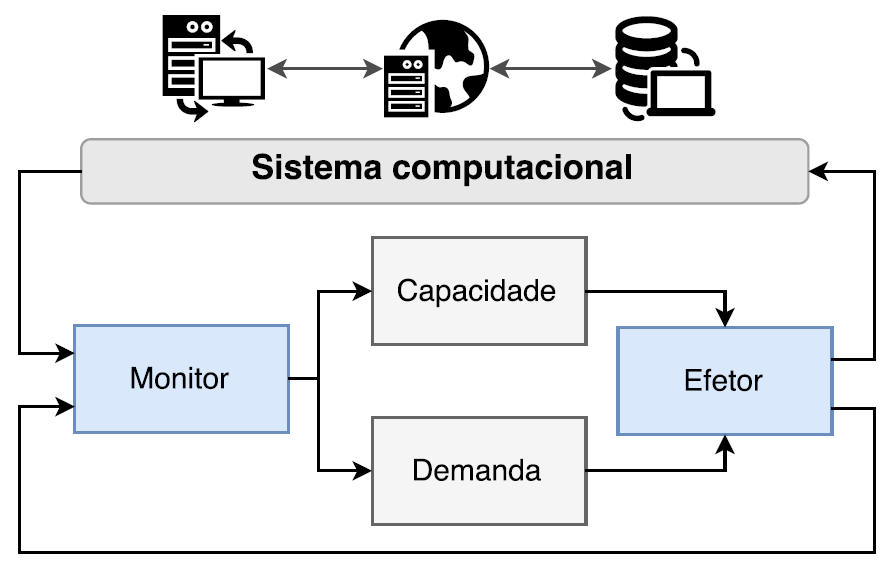
\includegraphics[scale=.4]{images/medc.png}
		\caption{MEDC: Monitor, Efetor, Demanda, Capacidade. \cite{Lourenco2015}}
		\label{fig:medc1}
	\end{figure}
\end{frame}

\begin{frame}{Modelo MEDC - o transiente}
	\begin{itemize}
		\item O transiente em um sistema computacional pode ser provocado por:
		\begin{itemize}
			\item Uma mudança na carga de trabalho 
			\item Uma mudança na capacidade interna (quantidade de recursos).
		\end{itemize}  
		\item O modelo MEDC mapeia esses dois aspectos nas responsabilidades respectivamente:
		\begin{itemize}
			\item \textbf{\textit{Demand} (modulação da carga)};
			\item \textit{Capacity} (modulação dos recursos).
		\end{itemize}
	\end{itemize}
\end{frame}



\begin{frame}{Modelo MEDC - demanda e capacidade}
	\note{no modelo MEDC diz que a ferramenta tem que incluir a pertubação de maneira programada realimentada (ex: quando a taxa de utilização ativem um nível)}
	\begin{itemize}
		%		\item O monitoramento produz as medidas para que a modulação de demanda e capacidade sejam feitas em tempo real;
		%		\begin{itemize}
		%			\item A saída do experimento deve produzir também gráficos temporais.
		%		\end{itemize}
		\item Uma perturbação pode ocorrer:
		\begin{itemize}
			\item Em função do tempo, (um acidente programado);
			\item Em função das medidas de desempenho, (de modo realimentado).
		
				\begin{itemize}
					\item \textbf{A modulação da carga} pode ser feita em função da \textit{taxa de requisições} (reduzir a carga admitida quando a utilização passar de certo limite).  
					\item \textbf{A modulação da capacidade} pode ser feita em função da utilização da CPU (aumentar os recursos quando a utilização ultrapassar certo patamar).  
				\end{itemize} 
		\end{itemize} 
	\end{itemize}
\end{frame}

%\begin{frame}{Modelo MEDC - Dinâmica}
%	\note{somente para completar o modelo, a capacidade e a demada dão os numeros mas quem atuaçõ é o Efector que é o mecanimos de atuação do Modelo}
%	\begin{itemize}
%		%		\item A modulação da demanda e a capacidade podem se refletir em: 
%		%		\begin{itemize}
%		%			\item política de admissão de carga;
%		%			\item gerenciamento de recursos.
%		%		\end{itemize} 
%		
%		\item A modelagem da dinâmica é responsabilidade do Efetor;
%		\begin{itemize}
%			\item O mecanismo pelo qual isso é implementado, fisicamente, pode \textbf{implicar em certa dinâmica}.
%			\item se a política de capacidade determina que os recursos devem ser aumentados, \textbf{o Efetor modela o atraso e a inércia} para a alocação e o desalocação dos recursos. 
%		\end{itemize}
%		
%	\end{itemize}
%\end{frame}



%\begin{frame}{O que é MEDC}
%	
%	\begin{columns}
%		\begin{column}{.4\textwidth}
%			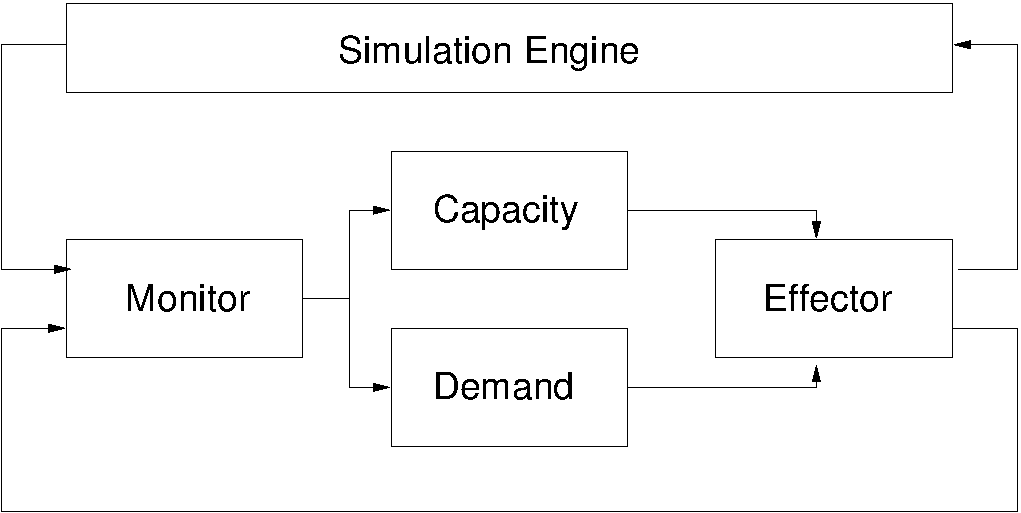
\includegraphics[width=.85\linewidth,valign=t]{../monograph/images/extension-block.pdf}
%
%		\end{column}
%		\begin{column}{.6\textwidth}
%			\textbf{"um conjunto de requisito que especificam uma arquitetura conceitual, intitulada MEDC (\textit{Monitor, Effector, Demanda and Capacity})."}
%			
%			\hfill-- Lourenço 2015
%		\end{column}
%	\end{columns}
%		
%	%\vspace*{10pt}
%	\begin{columns}
%		\begin{column}{0.9\textwidth}
%			\begin{itemize}
%				\item[\textit{Demand}:] referência para a capacidade de entrada e determinar a forma como a carga de trabalho muda ao longo do tempo;
%
%				\item[\textit{Capacity}:]  é a disposição análoga no que diz respeito aos recursos do sistema;
%				
%				\item[\textit{Monitor}:] sensor e aquisição de dados temporais, coletando os dados sobre o sistema e torná-lo disponível;
%				
%				\item[\textit{Effector}:] mecanismos de atuação através modulação, serve para a modelar os componentes operacionais que afetam a dinâmica \textit{Capacity} e \textit{Demand}.
%			\end{itemize}
%		\end{column}
%	\end{columns}
%\end{frame}

